\documentclass[../main.tex]{subfiles}

\begin{document}

\subsection{Models}

Our primary model for the experiments in this paper is the monotonic probit RBF-GP model described above. We also evaluate the same model without the monotonicity constraint in order to independently evaluate the benefit of monotonicity relative to the benefit of our novel acquisition function. To provide a fair comparison, this nonmonotonic model uses the exact same variational inference and rejection sampling procedure described above, except we accept all samples. Finally, we include an implementation of the separable linear-RBF model of Song and colleagues also described above, as this is the most closely related prior work to ours. Since no public implementation of this model is available to our knowledge, we use our own implementation, with one difference: we use variational inference (VI) rather than expectation propagation (EP). The use of a consistent inference algorithm makes for a fairer comparison with our models, but VI and EP can perform differently in different settings. Likely due to this change in inference approach, our results do not perfectly replicate that reported in the prior work.

GP kernels typically incorporate several hyperparameters that are fit to the data, typically to maximize marginal likelihood of the data. For the RBF kernel, the hyperparameters are the \emph{length scale}, which determines the distance in stimulus space for which points remain correlated, and the \emph{output scale}, which is an overall scale on function values. The linear kernel used in the additive model also has an output scale. As is standard practice in GP regression, we gave priors to these parameters to regularize the fitting and improve inference. Our objective for the output scale was to encourage the values of the latent psychometric field $f(x)$ to be in the operating range of the probit function, so we used a uniform prior between 1 and 4 (corresponding to covering response probabilities spanning a range of 0.84 in the lower end or 0.99997 in the upper end). Our objective for the lengthscale was to exclude lengthscales larger than the range of the data (since they are unidentifiable) or smaller than 10\% of the range of the data (since such highly irregular functions are unlikely in psychophysics). We thus used an inverse-gamma prior with parameters set such that 98\% of the probability mass was within this range.

\subsection{Optimizing the objective function}

For the nonmonotonic and monotonic full-RBF GPs, we optimize the acquisition function by stochastic gradient descent, since the use of rejection sampling makes the posterior stochastic and precludes the use second-order gradient methods that assume noiseless function evaluations. For the linear-additive model we include an additional heuristic proposed by \citet{Song2018} of adding noise to encourage exploration. For this heuristic, we first compute the acquisition function over a dense grid of points generated from a quasi-random Sobol sequence, normalize the values to be between 0 and 1, add a $\mathcal{N}(0, 0.2)$ random value to each, and pick the max of the noisy value. We confirmed that introducing this heuristic indeed helped to somewhat mitigate the boundary over-exploration effects we otherwise saw in that model (though as we will see below, these issues were not fully mitigated).

\subsection{Test functions based on audiometry data}
Previous applications of nonparametric psychophysics have focused primarily on the domain of psychoacoustics, specifically pure tone auditometry. To compare to this past work, we used the same set of test functions: the mean thresholds of 338 exemplars of four audiometric phenotypes defined from an animal model of age-related hearing loss. In all cases they define a hearing threshold in dB as a function of tone frequency (in kHz), measured from pure tone audiograms measured using standard audiometric procedures. Since no public implementations of these test functions is available, we followed the same procedure as \citet{Song2017b} to generate our own version: we first extracted ground-truth audiometric thresholds from Fig.~2 in \citet{Dubno2013}, and used cubic spline interpolation and linear extrapolation to evaluate them over the full range from 0.125 to 16 kHz\footnote{We thank the authors for their clarification by email about this procedure}. Then, to evaluate the latent psychometric field at any point we first interpolate/extrapolate the threshold from those measured values, and then use the standard linear model with that threshold. That is, $f_{song}(x_c, x_i) := \frac{x_i-\theta_{song}(x_c)}{\beta}$, where $x_i$ is the intensity value (in dB), $x_c$ is the context value (in kHz), $\theta(\cdot)$ is the interpolated threshold and $\beta$ is a psychometric spread parameter. As in previous work, we use all four phenotypes from \citet{Dubno2013} as test functions, and a grid of $\beta \in [0.2, 0.5, 1, 2, 5, 10]$. We plot the ground-truth threshold functions in Fig.~\ref{fig:audiometric-thresholds}.

\begin{figure}[htb]
  \centering
  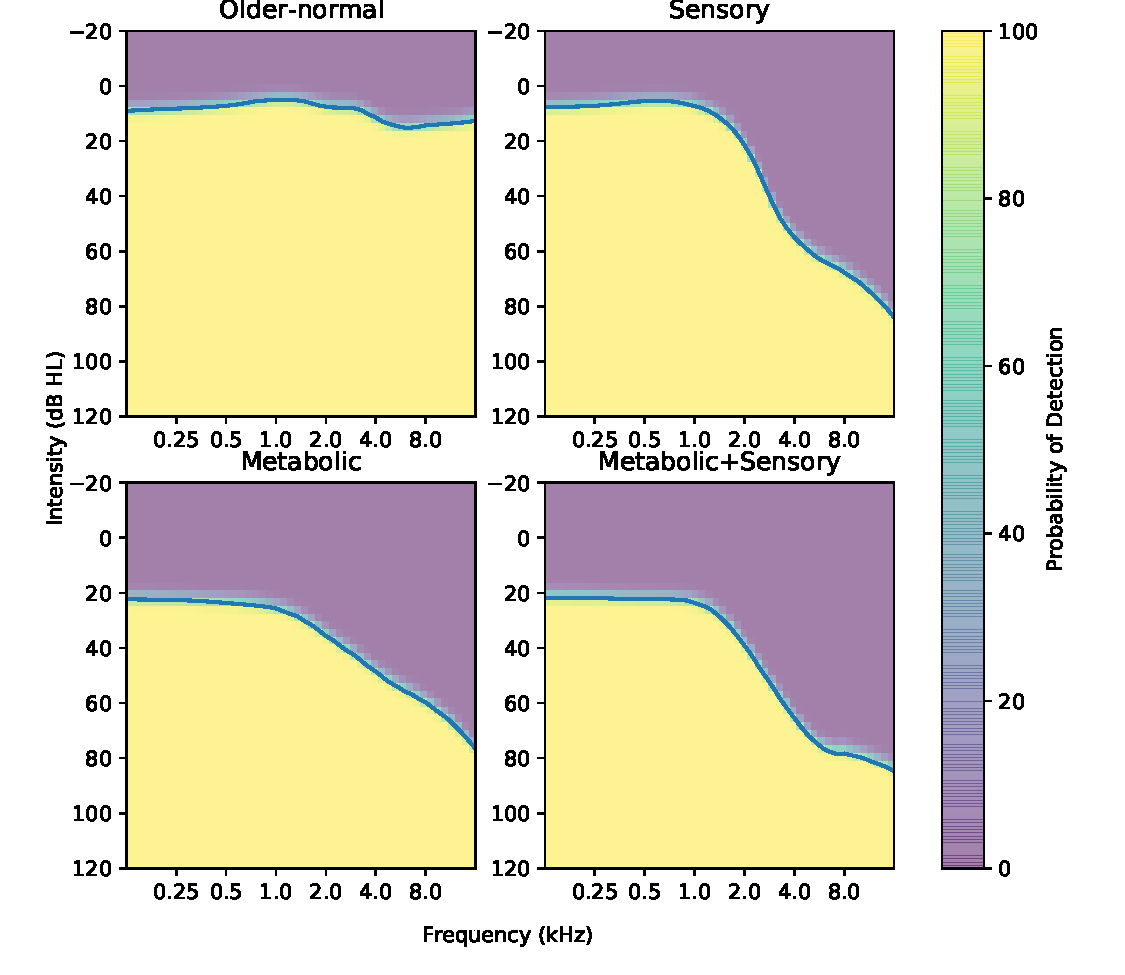
\includegraphics[width=0.95\columnwidth]{song_testfuns.pdf}
  \caption{\textbf{Audiometric test functions ground truth}. Surfaces generated with \protect{$\beta=2$} for the $f_{song}$ function described in the main text.}
  \label{fig:audiometric-thresholds}
\end{figure}

\subsection{New test functions for adaptive psychophysics}
The above test function, while based on real psychometric thresholds, makes a strong separability assumption between context and intensity: it assumes that the context does not interact with intensity but simply shifts the psychometric function. Furthermore, the empirically informed thresholds have fairly simple relationships with the contextual variable, all taking a sigmoid shape with large flat portions where context has minimal effect on the threshold. We introduce a novel, more difficult parametric test function for adaptive psychophysics, in two variants. First, we replace the interpolated context function with a fourth-order polynomial:

\begin{align}
  \theta_h(x_c) := 2(0.05 + 0.4(-1 + 0.2x_c)^2 x_c^2),
\end{align}

Next, we create a simple multiplicative interaction between the context and intensity dimensions. For a detection variant, we use the following transformation:
\begin{align}
  f_{det}(x_i, x_c) := 4\frac{1 + x_i}{\theta_h(x_c)} - 4,
\end{align}
which (after probit transformation) takes on the value of approximately 0 for 0 intensity. This matches standard detection experiments, where participants respond based on the presence of a stimulus. For a discrimination variant, we use:

\begin{align}
  f_{disc}(x_i, x_c) := 2\frac{1 + x_i}{\theta_h(x_c)},
\end{align}
which has response probability of 0.5 for 0 intensity. This matches standard discrimination experiments, where participants respond based on detecting a difference between pairs of stimuli. Both functions are visualized in Fig.~\ref{fig:novel-testfuns} over their input domain of $[-1, -1]$ to $[1, 1]$. In contrast to the audiometry test function, these psychometric functions depend on the context dimension over the entire domain. In addition, while they retain linearity in $x_i$, the interaction with context is now multiplicative, violating the separability assumption. While this test function is not directly drawn from real data, we think it provides a more realistic reflection of the complexities of psychometric data, especially in domains like haptics and multisensory perception.

\begin{figure}[htb]
  \centering
  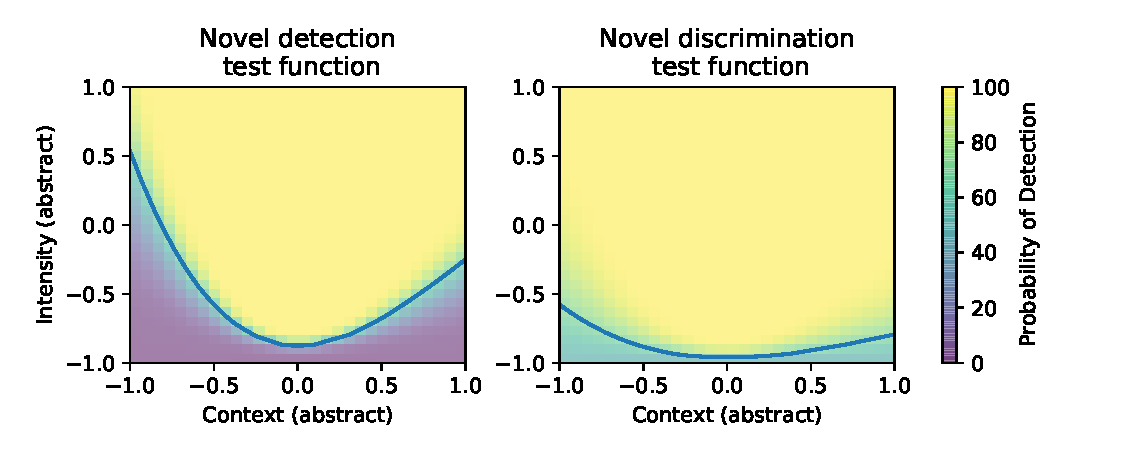
\includegraphics[width=0.95\columnwidth]{novel_testfuns.pdf}
  \caption{\textbf{Novel test functions for adaptive psychophysics}. On the left is the detection variant (response probability is approximately 0 at the lowest intensity), and on the right is the discrimination variant (response probability is 0.5 at the lowest intensity). The line marks the 0.75 threshold.}
  \label{fig:novel-testfuns}
\end{figure}

\subsection{Simulations}
Our simulation set was a full permutation over the following items:
\begin{itemize}
  \item Three model variants: the linear-additive GP model used in past work, a conventional probit-RBF GP, and the monotonic RBF GP.
  \item 26 test functions, consisting of [a] the two variants of our novel test function defined above (detection and discrimination), and [b] 24 audiometric test functions derived from the four phenotypes from Dubno and colleagues and the six noise levels previously used by Song and colleagues (0.2, 0.5, 1, 2, 5, and 10).
  \item Four acquisition functions: BALD, BALV, LSE, and the Thompson sampling variant of LSE (LSETS). We did not evaluate LSETS for the additive GP model because the noisy-acquisition heuristic is conceptually similar. We also included a Sobol acquisition baseline.
\end{itemize}

We initialized each simulation with 5 Sobol trials and ran it for 145 adaptive trials, for a total of 150 trials. In all cases our objective was to estimate the 0.75 threshold. Preliminary experiments with 20 Sobol trials showed the same patterns we report here, though they generally yielded slightly worse performance for the full RBF-based methods and better performance for the additive method (but again, the ordering of results was not changed by this for any test function). We repeated each simulation 100 times under different simulation seeds, for a total of 33800 simulations. The full set of simulations took about a week to run on a single 96-core workstation running on Amazon's EC2 cloud.

We made a conscious decision not to include classical methods: we did not include the method of constant stimuli because even the maximal trial counts we are considering here (150) are insufficient for this method, with trial counts in the 1000s needed for 2d spaces. We did not include parametric adaptive methods because, as noted above, they either have no way of scaling to higher dimensions except by using a grid (QUEST, PEST, etc) or require a parametric assumption for the effect of context that is not available a priori for any of our test functions (QUEST+).

\subsection{Evaluation}
For each simulation, we computed mean absolute error against the ground-truth response probability evaluated over a $30\times 30$ grid. We also evaluated the mean absolute error against the ground-truth threshold. Thresholds were computed by finding the two nearest points to the desired threshold for each value of the context dimension in the aforementioned grid, and performing local linear interpolation between those points to find the threshold. This was done identically to the ground truth function and the model-based estimate. We recorded additional performance metrics (correlation between true and estimated value, maximum absolute error, mean squared error) that showed the same patterns we report here.

\end{document}
